% THIS IS SIGPROC-SP.TEX - VERSION 3.1
% WORKS WITH V3.2SP OF ACM_PROC_ARTICLE-SP.CLS
% APRIL 2009
%
% It is an example file showing how to use the 'acm_proc_article-sp.cls' V3.2SP
% LaTeX2e document class file for Conference Proceedings submissions.
% ----------------------------------------------------------------------------------------------------------------
% This .tex file (and associated .cls V3.2SP) *DOES NOT* produce:
%       1) The Permission Statement
%       2) The Conference (location) Info information
%       3) The Copyright Line with ACM data
%       4) Page numbering
% ---------------------------------------------------------------------------------------------------------------
% It is an example which *does* use the .bib file (from which the .bbl file
% is produced).
% REMEMBER HOWEVER: After having produced the .bbl file,
% and prior to final submission,
% you need to 'insert'  your .bbl file into your source .tex file so as to provide
% ONE 'self-contained' source file.
%
% Questions regarding SIGS should be sent to
% Adrienne Griscti ---> griscti@acm.org
%
% Questions/suggestions regarding the guidelines, .tex and .cls files, etc. to
% Gerald Murray ---> murray@hq.acm.org
%
% For tracking purposes - this is V3.1SP - APRIL 2009

\documentclass{acm_proc_article-sp}

\usepackage{multirow}
\usepackage{subfigure}
\usepackage{graphicx}
\usepackage{graphics}
\usepackage{rotating}
\usepackage{verbatim}
\usepackage{float}
\usepackage{url}

\usepackage{listings}
\usepackage{color}
\definecolor{javared}{rgb}{0.6,0,0} % for strings
\definecolor{javagreen}{rgb}{0.25,0.5,0.35} % comments
\definecolor{javapurple}{rgb}{0.5,0,0.35} % keywords
\definecolor{javadocblue}{rgb}{0.25,0.35,0.75} % javadoc
 
\lstset{language=Java,
basicstyle=\ttfamily,
keywordstyle=\color{javapurple}\bfseries,
stringstyle=\color{javared},
commentstyle=\color{javagreen},
morecomment=[s][\color{javadocblue}]{/**}{*/},
%numbers=left,
numberstyle=\tiny\color{black},
stepnumber=2,
numbersep=10pt,
tabsize=4,
showspaces=false,
showstringspaces=false}



\restylefloat{table}
\hyphenation{op-tical net-works semi-conduc-tor}
\begin{document}

\title{Automated Discovery of Failure Domain}

\numberofauthors{2} %  in this sample file, there are a *total*
% of EIGHT authors. SIX appear on the 'first-page' (for formatting
% reasons) and the remaining two appear in the \additionalauthors section.
%
\author{
% You can go ahead and credit any number of authors here,
% e.g. one 'row of three' or two rows (consisting of one row of three
% and a second row of one, two or three).
%
% The command \alignauthor (no curly braces needed) should
% precede each author name, affiliation/snail-mail address and
% e-mail address. Additionally, tag each line of
% affiliation/address with \affaddr, and tag the
% e-mail address with \email.
%
% 1st. author
\alignauthor
Mian Asbat Ahmad\\
       \affaddr{Department of Computer Science}\\
       \affaddr{University of York}\\
       \affaddr{York, United Kingdom}\\
       \email{mian.ahmad@york.ac.uk}
% 2nd. author
\alignauthor
Manuel Oriol \\
       \affaddr{Department of Computer Science}\\
       \affaddr{The University of York}\\
       \affaddr{York, United Kingdom}\\
       \email{manuel.oriol@york.ac.uk}
}


\maketitle
\begin{abstract}
Many research studies in the random testing literature refer to 
point, block and strip fault domains across the input domain of a system.
A number of new strategies have also been devised on this principle claiming better results.
However, no study was conducted to graphically show their existence
and the frequency of each faulty domain in real production application. 

In this research we study fault domains and check to which type of domains they belong. 
Our experimental results show that in 60\%  cases faults form point domain, 
while block and strip domain form 20\% each. We also checked what relation exists 
between fault domains traced back to only one fault: are they contiguous, separate, or marginally adherent. 

This study allows for a better understanding of fault domains and assumptions made on the 
strategies for testing code. We applied our results by correlating our study with three random strategies: random, random+ and DSSR. 

\end{abstract}

%A category including the fourth, optional field follows...
\category{D.2.5}{Software Engineering}{Testing and Debugging}[Testing Tools, Failure Domains, Random testing, Automated Testing]

\section{Introduction}\label{sec:intro}

Testing is fundamental requirement to assess the quality of any software. Most if not all, modern testing techniques execute the System Under Test (SUT) with specific input 
and compare the obtained results against the test oracle. A report is generated at the end of each test session which contain any 
discovered faults with the input values, which lead to the generation of the fault. These reports are later evaluated by
debuggers to fix the discovered faults. The system is given back to the testers to find more faults for rectification. This process is continue until a certain level of satisfaction is reached.\\

It is important to note that these techniques only identify the instance of failure and don't focus on the  failure domain. This research can decrease the overall testing times by reducing the number of code exchanges between testers and debugger. It is achieved by tracking the failure domain and not only a single instance failure. Tracking failure domain provide more information about the behaviour of the fault.

%that also served as regression testing. None of the testing techniques evaluate the nature of the fault and the pattern in which the fault reside. 


%The aim of this research study is to find not only find the values for which the system fails but also the domains of failure causing inputs which will help in automated generation of fault targeted test cases for any black-box testing technique.\\

%Random testing is a black-box testing technique in which parts (methods/modules) of SUT are selected randomly and then executed against randomly generated test data according to the required type from the whole input domain. Results obtained from the execution are either compared to the specifications of the SUT or language exceptions which served as a test oracle. Any test output that fail to meet the oracle either because of failing to comply the specification or trigger the exceptions are considered as potential faults. The same report is used by the testers for debugging and regression testing.\\

%Over the past few years there is a tremendous growth in development of hardware whose main focus is to increase the computer processing power. The computers that served as a mini and mainframe computers few years ago are turned into personal computer in todays modern age. To utilise this processing power various software development companies started to develop more sophisticated and processing hungry softwares. These softwares provide simple and easy to use Graphical User Interface (GUI) but on the back end they are equally complex and consist of thousands of instructions. This increase in size of the software also increases the difficulty of preserving high quality, reliability, portability, maintainability and efficiency of the software. These problems are mainly cater by software testing. The increase of complexity and size of softwares also forced the researchers to find new ways of software testing that are more efficient, reliable and speedy to cope with the ever increasing hardware and software industry.\\

Chan et al.  \cite{Chan1996}  found domains of failure causing inputs across the whole input domain.
They divided them into block, strip and point domain as shown in Figure \ref{fig:patterns}. They further suggested that the effectiveness of proportional sampling strategy can be improved by taking into account the possible characteristics of failure causing inputs.

\begin{figure}[htp]
\centering
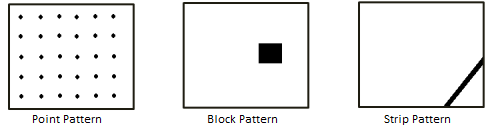
\includegraphics[width=8cm,height=2.5cm]{ART_Patterns.png}
\caption{Failure domains across input domain \cite{Chan1996}}
\label{fig:patterns}
\end{figure}

In search of better testing results Chen et al., implemented the same idea in Adaptive Random Testing (ART) \cite{Chen2008}. In ART test data is generated by selecting test values farthest away from one another to increase the chance of hitting these faulty domains. The experiments performed using ART showed up to 50\% better results as compared to the traditional/pure random testing which has no criteria for input selection. Mirror Adaptive Random Testing (MART)  \cite{Chen2003}, 
Feedback-Directed Random Testing (FDRT) \cite{Pacheco2007}, 
Restricted Random Testing (RRT) \cite{Chan2002} and Quasi Random Testing  (QRT) \cite{Chen2005} 
are the strategies based on the same principle that found better results compared to ordinary random testing.

Significant research has been done to utilise the failure domains 
but their existence, nature and boundaries need further attention. 
In this article we present an automated random technique to discover 
and investigate the failure domains across the input domain. 
Having this information prior to testing enables the tester to guide testing according 
to the failure domain of the SUT, for example pure random testing is more effective 
for point domain than block and strip domains where as ART, MART, FDRT, RRT 
and QRT are more effective for block and strip fault domains than point fault domain.

%In our previous research we extended the same idea of the existence of different domains of failure across the whole input domain proposed by Chen et al, \cite{Chen2008} and accepted by various other researchers to develop a new strategy called Dirt Spot Sweeping Strategy [X]. However the experimental results showed not very considerable improvement then what we predicted. We performed 500 experiments in which we carried out 10000 tests but the results showed only 5\% improvement contrary to our prediction of 30\%. All the experiments were performed from a pool of open-source projects bundled in a repository called Qualitas Corpus \cite{Tempero2010}. Corpus contains more than 100 open-source java projects and maintained only for the purpose of unbiased research experiments. Therefore one of the conclusions derived from our experiments was that the patterns of failure may not exist in most of the software’s due to which our strategy which focus on these patterns didn’t produce much efficiency.\\
%It was therefore very interesting for us to do further research to find about the existence and nature of these failure patterns. Our main focus in this research paper is to discover whether there exist failure patterns across the input domain or not and if they exist then how frequent and what pattern they follow.\\

In Section II, we describe the automated technique of  discovering failure domains and explain its structure and function with the help of a flowchart and motivating example. Section III presents its implementation in automated random testing tool called York Extensible Testing Infrastructure (YETI). Section IV and V report the experiments performed using the proposed technique and evaluate \& discuss the obtained results. Section VI and VII discuss any threats to validity and related discussion. Finally we conclude in Section VIII. 

%The rest of this paper is organized as follows. The sections, II to X, describe automated strategy, Implementation, Experimental setup and analysis, Evaluation, Experimental results, discussion, conclusion and future work respectively.\\

\section{Problems and Solutions}\label{sec:probl_and_sol}
This paper address five. main problems in random testing. These are (1) Finding the whole domain of fault instead of only failing values, (2) Representation of fault values, (3) automation of the evaluation process, (4) Identification of fault domain for multi arguments methods and its representation, (5) Generation and classification of test values for Strings and complex (non scaler) arguments. This section elaborate each of the above mention problem and describe our proposed solution (if any) to them.

\subsection{Finding the whole domain of fault instead of only failing values}
Most of the testing tools take into account only the fault finding values with out giving due consideration to the domain in which the values exist. \subsection{Representation of fault values and fault domains}
points: instead of dumping logs and more complex reports we describe the fault domains with the help of charts. 
\subsection{Automation of the testing process}
We developed an automated system to test the system, generate the fault domain finding files, compile and execute them to find the fault domains if any. points: automation is achieved by combining the test tool and evaluation system e.g. yeti and ADFD.   
\subsection{Identification and representation of multi arguments data}
I think it is beyond the scope of this study to identify and represent more then 3 arguments method because at the moment we can show only three diminutional charts.
\subsection{Generation and classification of test values for string and complex (non scaler) arguments}
It is difficult to find the domain for strings and complex (non scaler) data therefore they can be exempted from this study.


\section{Automated Discovery of Failure Domain}\label{sec:adfd}

Automated Discovery of Failure Domain (ADFD) strategy is a new technique that find a failure domain across the whole input domain in an automated fashion. The discovered failure domains are presented in the form of graphs at the end of the session. The process is divided into the following four major parts for simplification. Each part is explained below.

\begin{enumerate}
\item Use of automated testing tool to find the failure in the given SUT.
\item Automated generation of modules at run time according to the found failure.
\item Automated compilation and execution of the generated modules.
\item Analysis of results obtained and graphically plot the fault domain .\\
\end{enumerate}


\begin{figure}[htp]
\centering
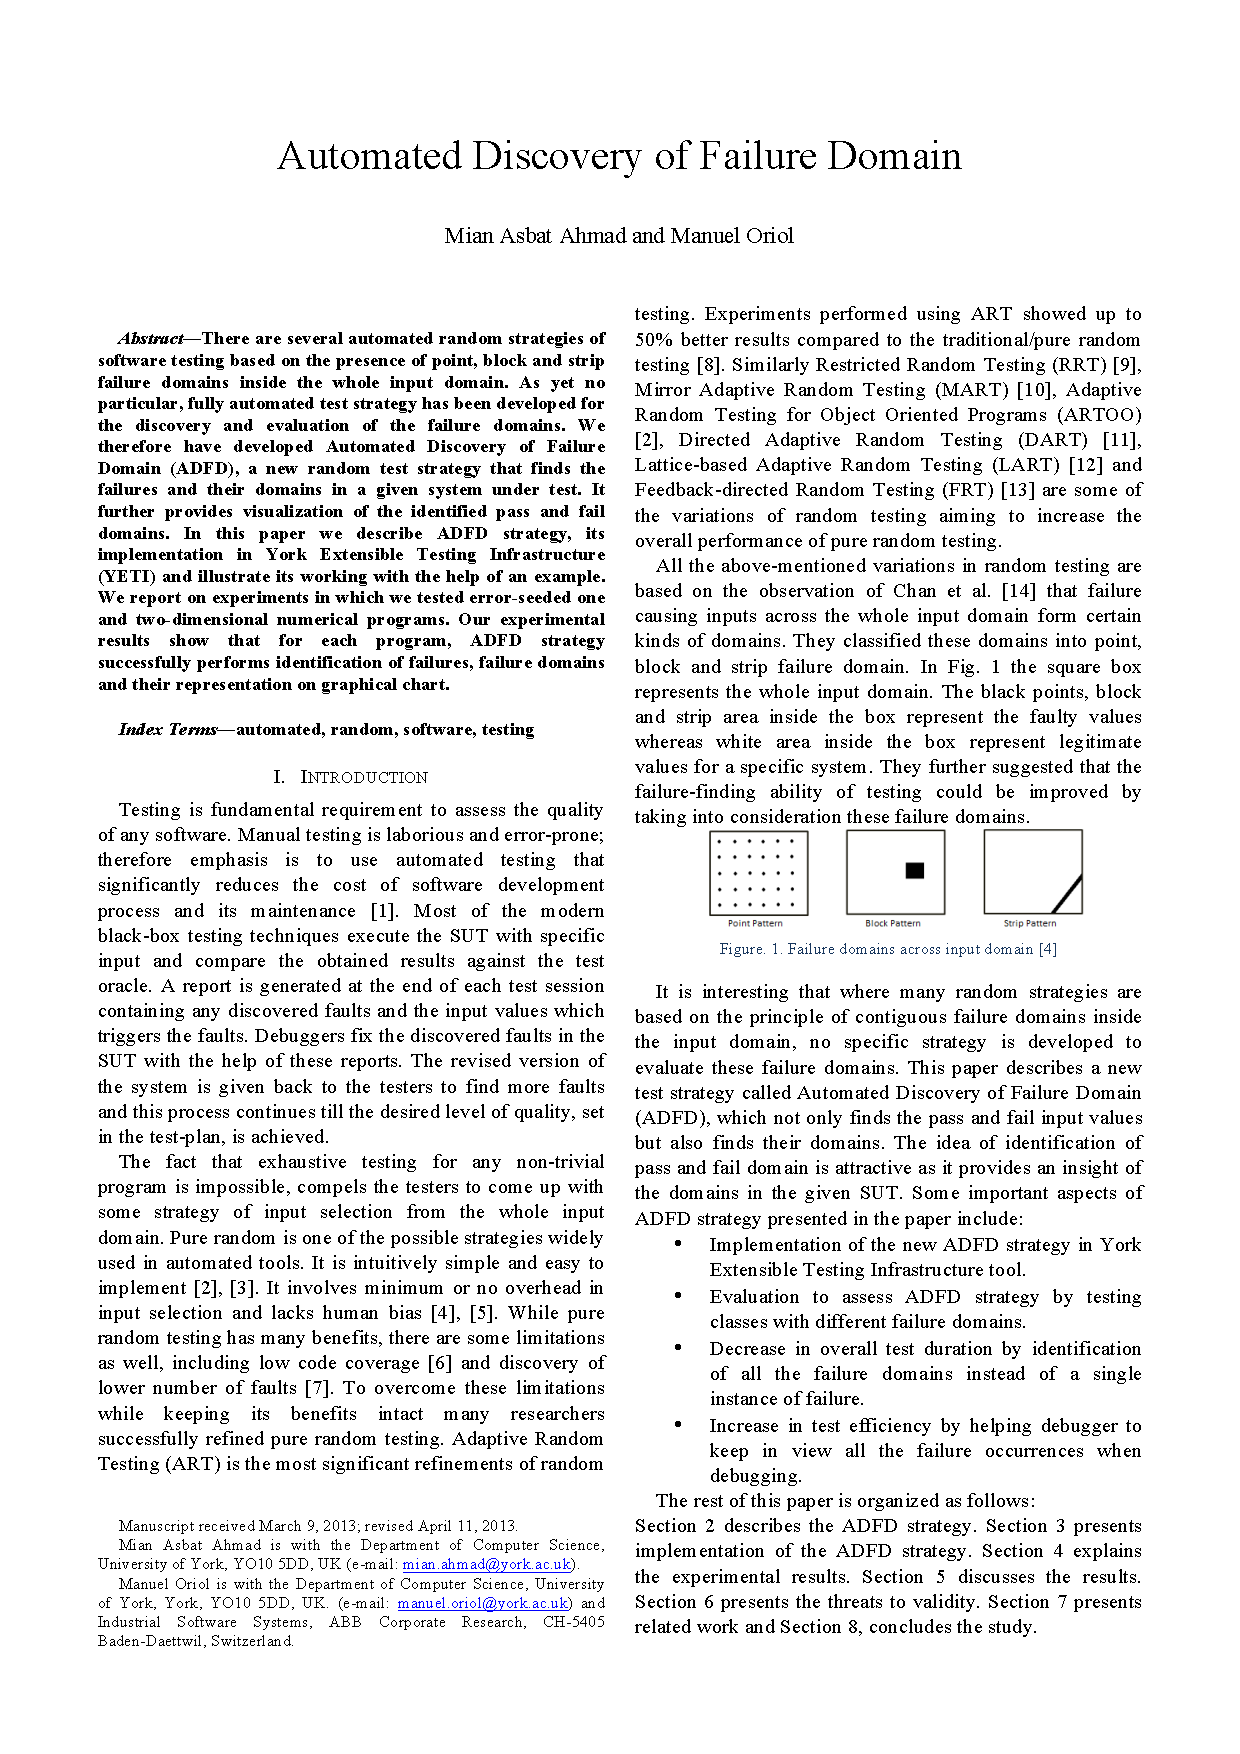
\includegraphics[width=5cm,height=4cm]{ADFD.png}
\caption{GUI of ADFD strategy}
\label{fig:patterns}
\end{figure}




\noindent \textbf{Automated testing to find the fault in given SUT:}\\*
\indent To find the failure domain for a specific fault first we need to identify the fault in the system. This required fault can be identified by manual testing but we selected automated testing system because it can saves time, resource and produce quick results. For this purpose we could select any automated testing system because the research is focusing on the failure domains and not on the performance of finding faults and for that reason F-measure, E-measure and P-measure etc were not of particular concern. York Extensible Testing Infrastructure (YETI) is selected to test and find the fault in given SUT mainly for its simplicity, speed and proven capability of finding potentially hazardous faults in many systems. It is a complete automated testing system that is capable of calling millions of instructions in one second on Java code. It is also capable of testing VB.Net, C, JML and CoFoJa beside Java. YETI was executed with its default strategy of random testing for finding the fault in our experiments.\\

\noindent \textbf{Automated generation of modules at run time according to the fault found:}\\*
\indent After finding the fault in the given SUT through an automated system we needed to write one, two or many modules based on the condition of the found fault. These modules are later executed to explore the nature of the failure domain for the found fault. To keep this process automated we used Java feature of generating dynamic code which is available in javax.tools package in Java language. We added additional functionality in YETI and now when the fault is found by YETI in the given SUT it stops testing and dynamically generate the required modules with .java extension and saves it to a file for further execution. This generated module can have one or more argument constant and one argument as variable.\\

\noindent \textbf{Automated compilation and execution of these modules:}\\*
\indent The testing process stops after the generated modules are written to a file with .java extension on some permanent media. A script is executed and the .java files produced earlier are fist compiled to get the binary .class file and then executed. During execution the static arguments of the module remain the same but the variable argument receive all the values of the whole input domain of that particular type. Once the execution of the generated modules is completed the results are produced by the system on the standard output.\\

\noindent \textbf{Generation of results and analysis:}\\*
\indent All the generated modules are executed by the system and the results obtained are saved and analysed. On the basis of analysis of these results we can identify that which particular domain that fault belongs to. If the module output a single value after few thousands of values then the fault belongs to the point domain. If it fails for a pool of value at some specific interval then it belongs to the block domain and if it fails to a large pool of continuos values than it belongs to a strip domain.\\

\subsection{Flow Chart of the process}

The following flow chart clearly identify the workflow of the whole process and the various steps involved in the process.

\begin{figure}[htp]
\centering
\includegraphics[width=8cm,height=12cm]{automatedFail.png}
\caption{Automated discovery of Failure Domain}
\label{fig:autofail}
\end{figure}


\section{Motivating Example}\label{sec:example}
The goal of ADFD is to find the fault in the SUT and its existence across the complete domain in an automated way. This helps the developers to debug the code keeping in view its every occurrence that may otherwise go unnoticed.
Published programs from literature \cite{Chen2003}\cite{Chan1996}\cite{Chen2004} of point, block and strip failure patterns are tested to explain the working of ADFD . These programs were translated in to java language for this experiment (See appendix 1 for more details). \\
%ADFD is a two step process where first step is to test the program through YETI and the second step is to execute the programs generated at the end of the first step. 

\begin{lstlisting}
/** 
* Calculate square of given number 
* and verify results. 
* The code contain 3 faults.
* @author (Mian and Manuel)
*/
public class Math1 {
 public void calc (int num1) {
  // Square num1 and store result. 
  int result1 = num1 * num1;
  int result2 = result1 / num1; // 1
  assert Math.sqrt(result1) == num1; // 2
  assert result1 >= num1; // 3
 } 
}
\end{lstlisting}

In step one each program was tested individually by YETI that discovered the existing faults and generated relevant program for each fault. The number of generated programs depend on the dimension of the program under test. Since all selected programs were two dimensional (containing two parameters) therefore two programs were generated for each found fault. Table \ref{tb:failtable} shows the programs generated and pass \& fail patterns discovered for each fault. For each test entire integer range i.e. -2147483648 to 2147483647 was selected as input domain.\\


%\begin{center}
\begin{table*}[t]
%\renewcommand{\arraystretch}{2}
\centering
%{\small} %normalsize

\begin{tabular}{|c|c|l|l|l|}

\hline 

\textbf{S. No}		& \textbf{Failure Pattern}	& \textbf{Specific Fault}	 		& \textbf{Pass Pattern} 			& \textbf{Fail Pattern} 			\\ \hline 


\multirow{2}{*}{1} 	&\multirow{3}{*}{Point}	&\multirow{2}{*}{Prog1.test1(i)}	& 00 to 00				&\multirow{2}{*}{0}	  			\\ \cline{4-4} 
				&					&							&00 to 00				&	                           			\\ \cline{3-5} \hline
\multirow{2}{*}{2} 	&\multirow{3}{*}{Block}	&\multirow{2}{*}{Prog2.test2(i)}	&00 to 00				&\multirow{2}{*}{0}	  			\\ \cline{4-4} 
				&					&							&00 to 00				&	                           			\\ \cline{3-5} \hline
\multirow{2}{*}{3} 	&\multirow{3}{*}{Strip}	&\multirow{2}{*}{Prog3.test3(i)}	&00 to 00				&\multirow{2}{*}{0}	  			\\ \cline{4-4} 
				&					&							&00 to 00				&	                           			\\ \cline{3-5} \hline
\end{tabular}
\caption{Failure domain with respect to one dimensional program}
\label{tb:failtable}
\end{table*}
%\end{center}




%\begin{center}
\begin{table*}[t]
%\renewcommand{\arraystretch}{2}
\centering
%{\small} %normalsize

\begin{tabular}{|c|c|l|l|l|}

\hline 

\textbf{S. No}		& \textbf{Failure Pattern}	& \textbf{Specific Fault}	 		& \textbf{Pass Pattern} 			& \textbf{Fail Pattern} 			\\ \hline 


\multirow{3}{*}{1} 	&\multirow{3}{*}{Point}	&\multirow{2}{*}{Prog1.test1(-4,i)}	&-2147483648 to -1				&\multirow{2}{*}{0}	  			\\ \cline{4-4} 
				&					&							&1 to 2147483647				&	                           			\\ \cline{3-5}
				&					&Prog1.test1(i,0)				&None						&-2147483648 to 2147483647 	\\ \hline
\multirow{4}{*}{2}	&\multirow{4}{*}{Block}	&\multirow{2}{*}{Prog2.test2(i,10)}	&-2147483648 to 9				&\multirow{2}{*}{10, 11}			\\ \cline{4-4} 
				&					&							&12 to 2147483647				&		   		   			\\ \cline{3-5} 
				&					&\multirow{2}{*}{Prog2.test2(10,i)}	&-2147483648 to 9				&\multirow{2}{*}{10, 11, 12}		\\ \cline{4-4} 
				&					&							&13 to 2147483647				&							\\ \hline
\multirow{5}{*}{3} 	&\multirow{5}{*}{Strip}	&\multirow{3}{*}{Prog3.test3(i,4)}	&-2147483648 to -2147483641	&-2147483640 to -214783637 		\\ \cline{4-5} 
				&					&	 						&-2147483636 to 7				&\multirow{2}{*}{8 to 11}			\\ \cline{4-4} 
				&					&	 						&12 to 2147483647				&							\\ \cline{3-5} 
				&					& \multirow{2}{*}{Prog3.test3(10,i)}	&-217483648 to 1				&\multirow{2}{*}{2 to 9}			\\ \cline{4-4}
				&					&	 						&10 to 2147483647				&							\\ \hline
\end{tabular}
\caption{Failure domain with respect to two dimensional program}
\label{tb:failtable}
\end{table*}
%\end{center}


In step 2 the generated programs were executed in such a way that the variable parameter receives all the values between -2147483648 to 2147483647 while static parameter remain constant. Results of the execution are demonstrated with the help of the following graphs. The graphs only scales to 100 values and not for complete integer range only to keep the fault patterns visible and more readable.

%We found that it is better for the developer to see the range because the fault can be found once but it can generate errors at multiple locations.like point pattern in the first graph only generate fault at location 0 but if the same zero is assigned to second argument then the whole domain values can fail.\\


\begin{figure}[htp]
\centering
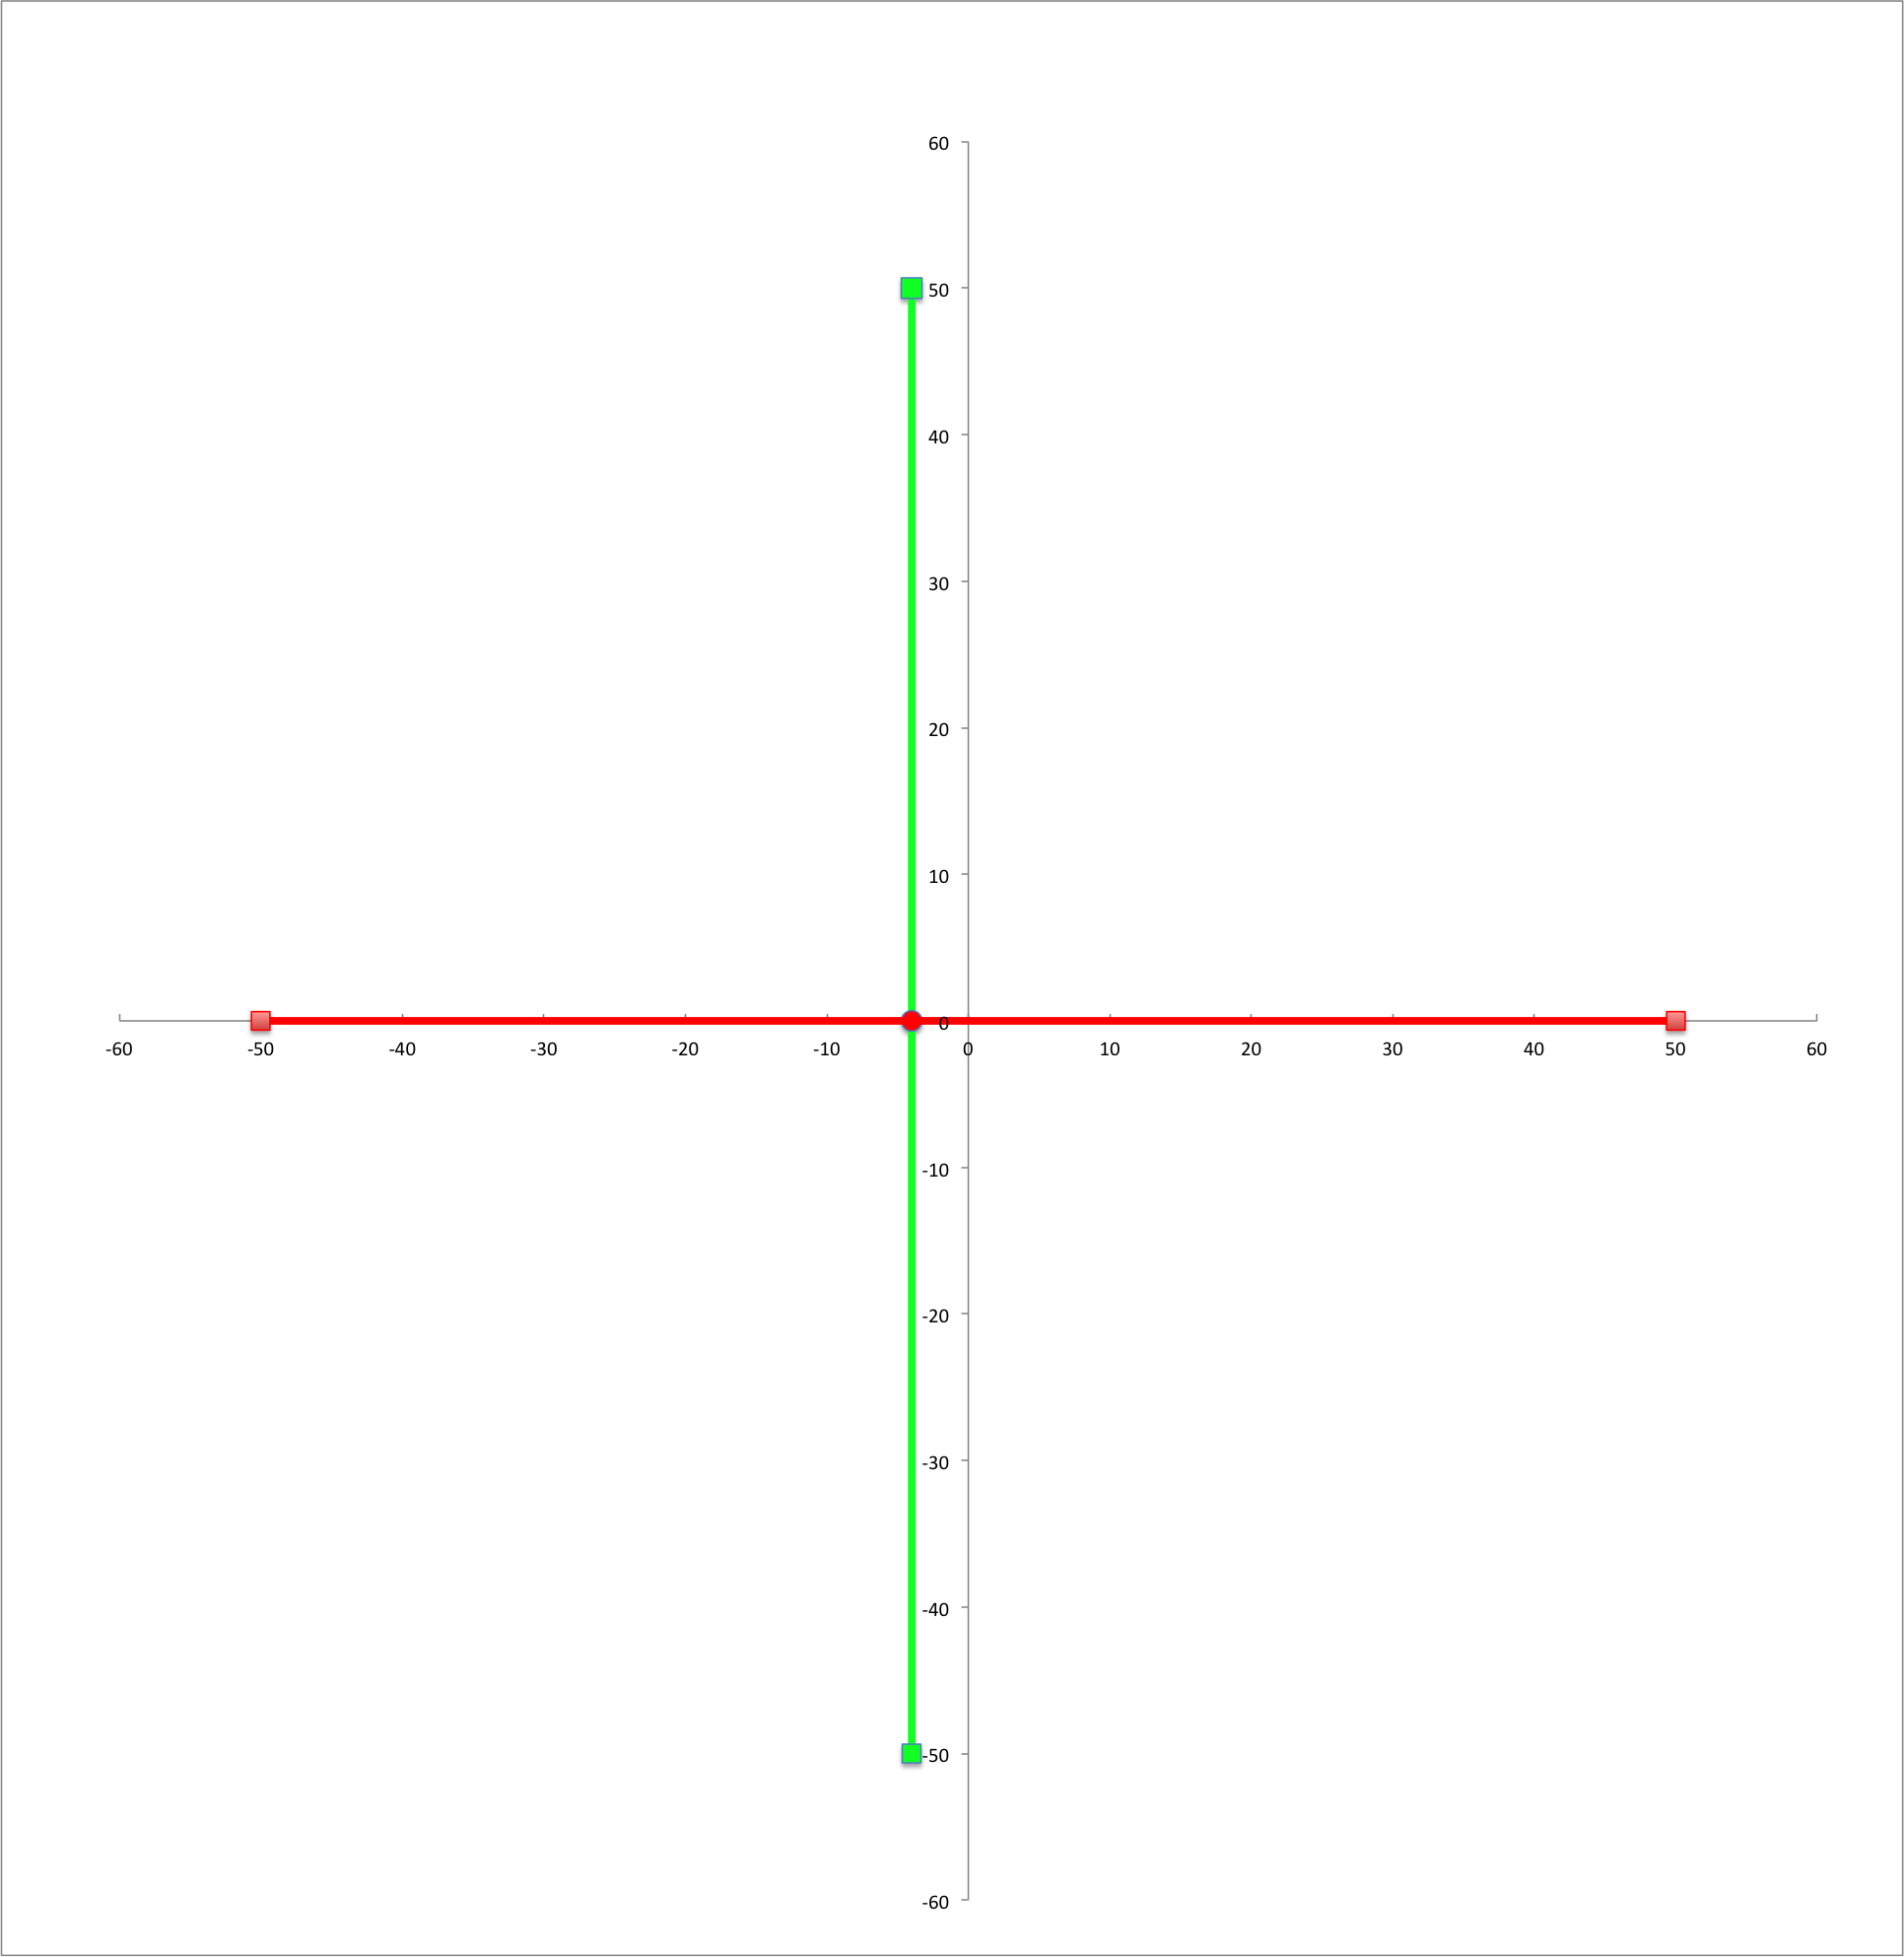
\includegraphics[width=4cm,height=4cm]{point_pattern.png}
\caption{Point pattern failure domain}
\label{fig:patterns}
\end{figure}


%Figure \ref{fig:point} shows the example of point pattern. In sub figure \ref{fig1:a} test only fails for 0 out of the whole integer range where as in sub figure \ref{fig1:b} all test fails when static variable is assigned with 0 value.


\begin{figure}[htp]
\centering
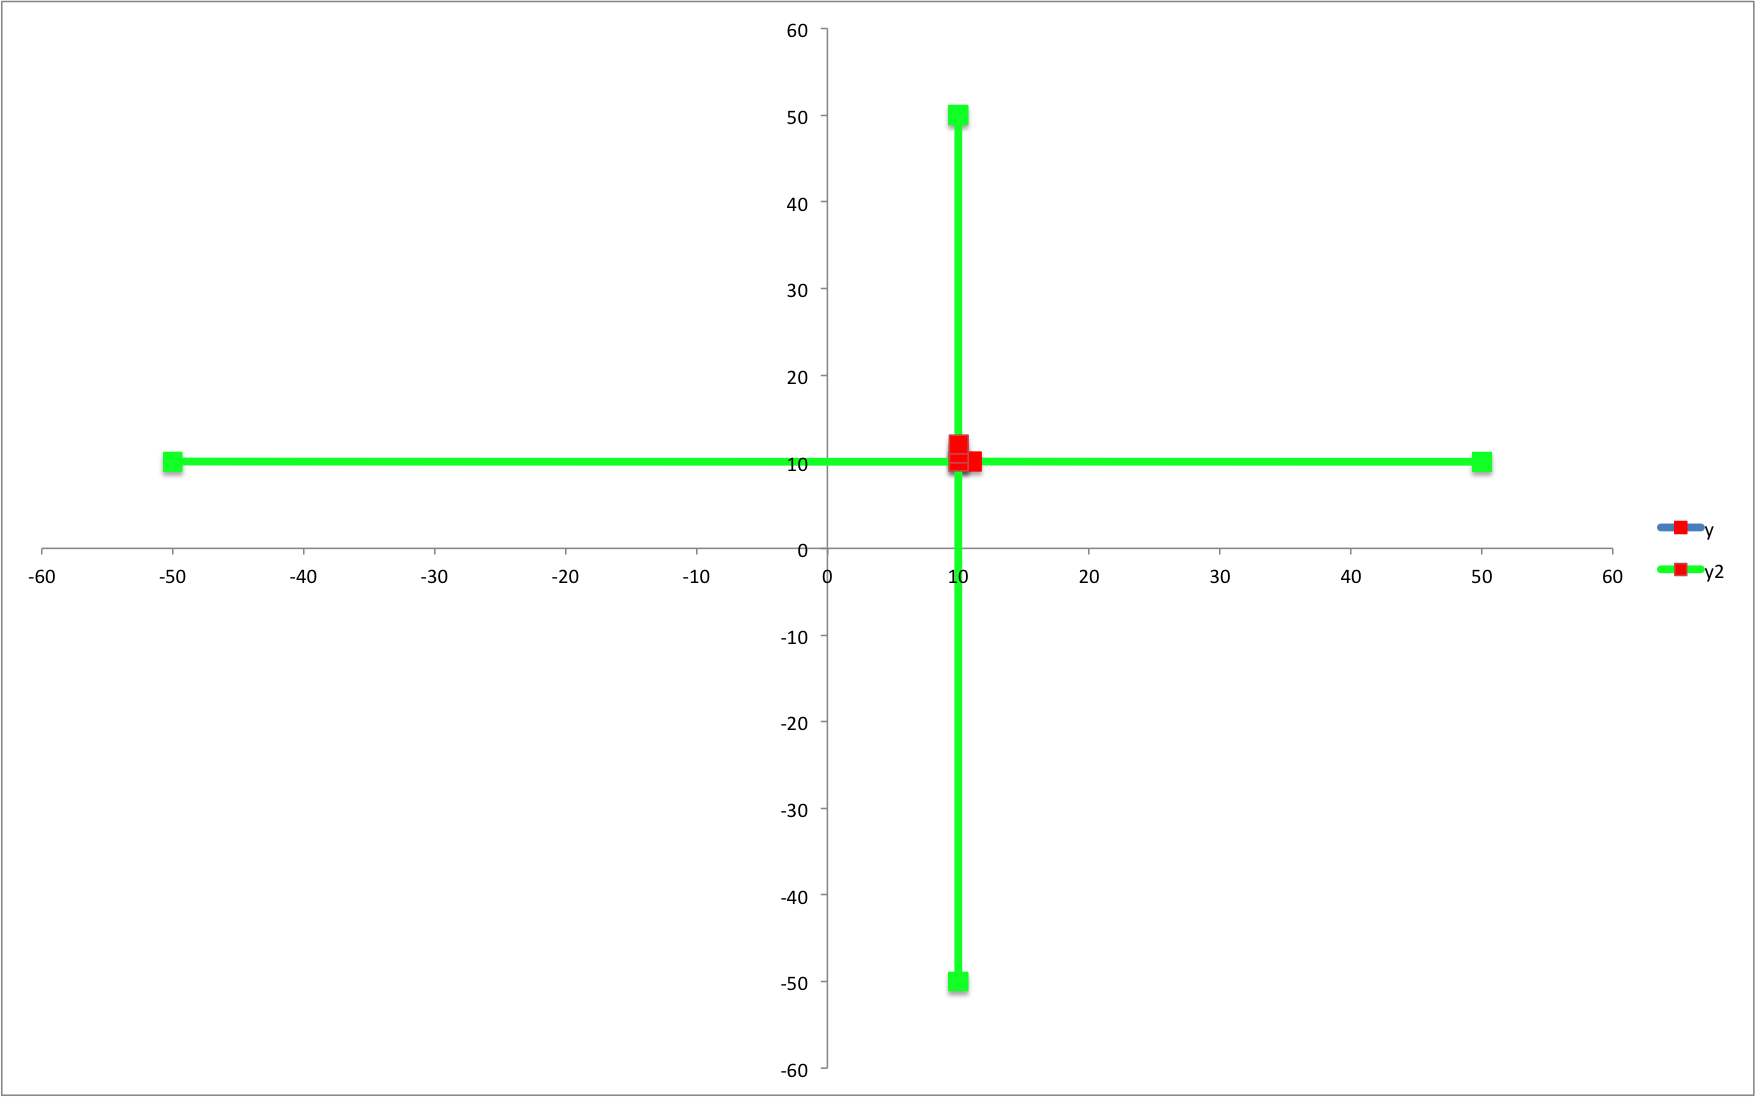
\includegraphics[width=4cm,height=4cm]{block_pattern.png}
\caption{Block pattern failure domain}
\label{fig:patterns}
\end{figure}


%Figure \ref{fig:block} shows the example of block pattern. Both sub figure \ref{fig1:a} and \ref{fig1:b} shows the block pattern of failure. The failure values are given in table \ref{tb:failtable}.

%\begin{figure}[htp]
%\centering
%\begin{center}
%  % Maximum length
 %\subfloat[Test 1 A]{\label{fig1:a}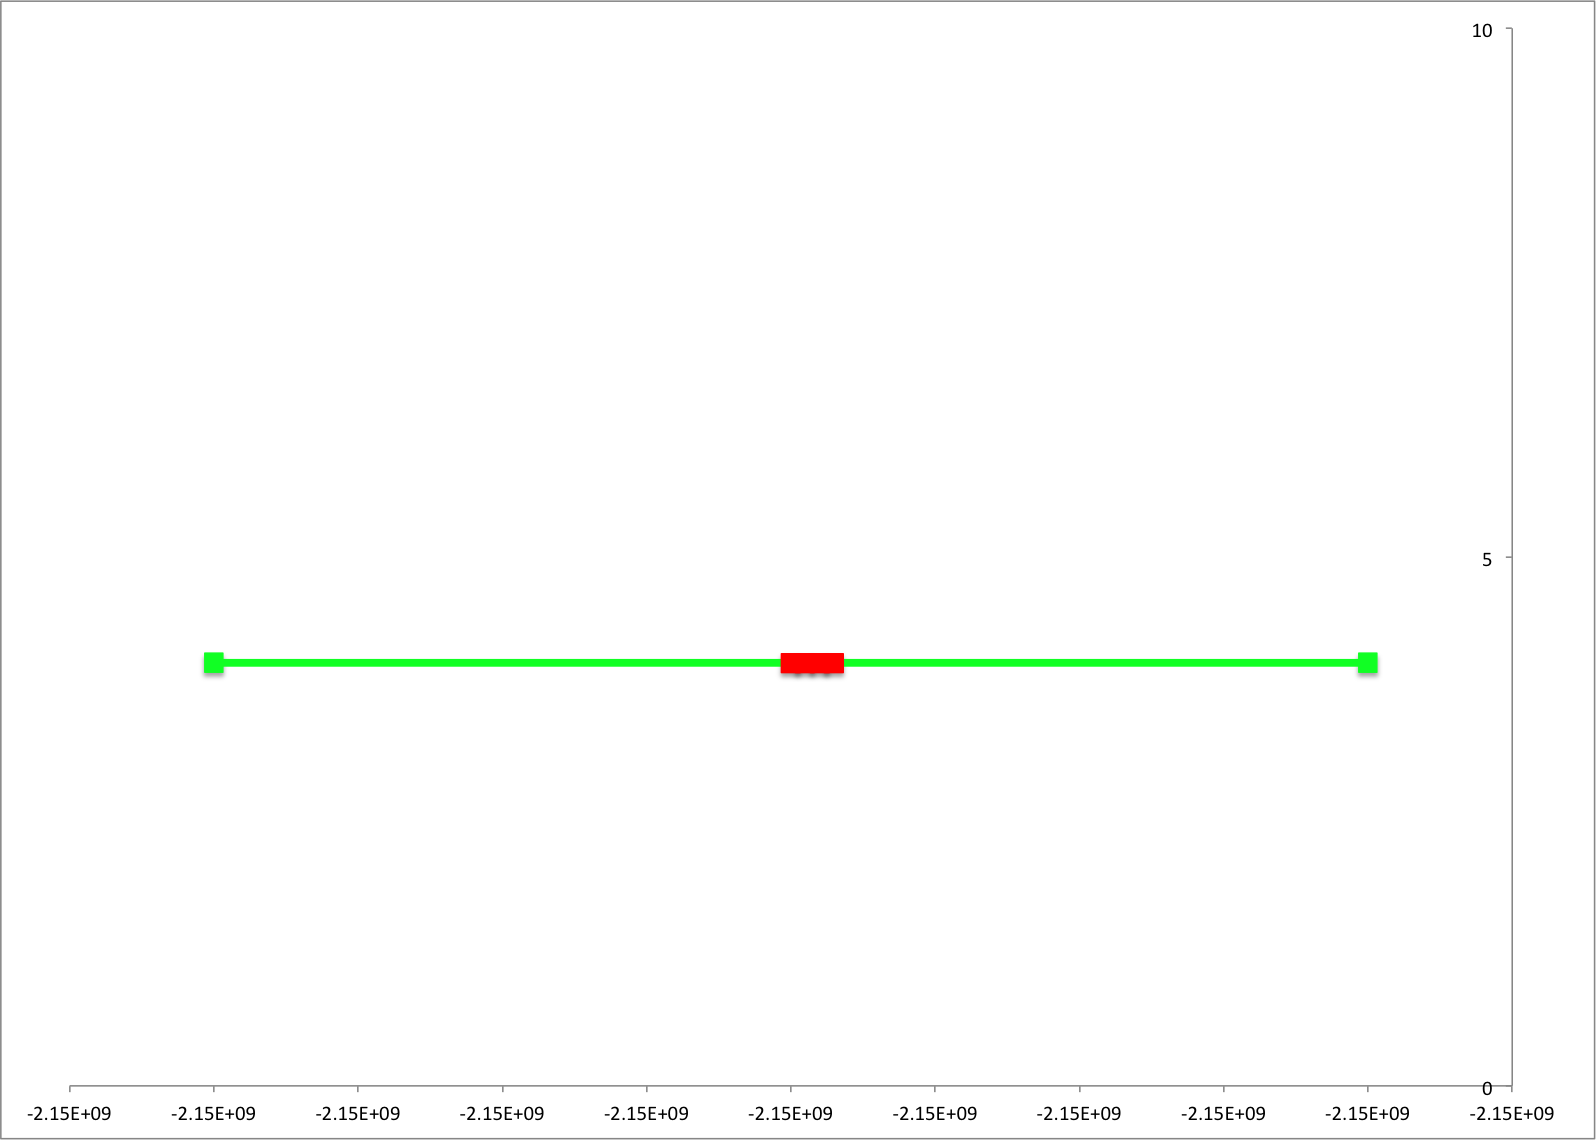
\includegraphics[width=0.49\linewidth]{excel_png/strip_pattern_B.png}}\hfill
 %\subfloat[Test 1 B]{\label{fig1:b}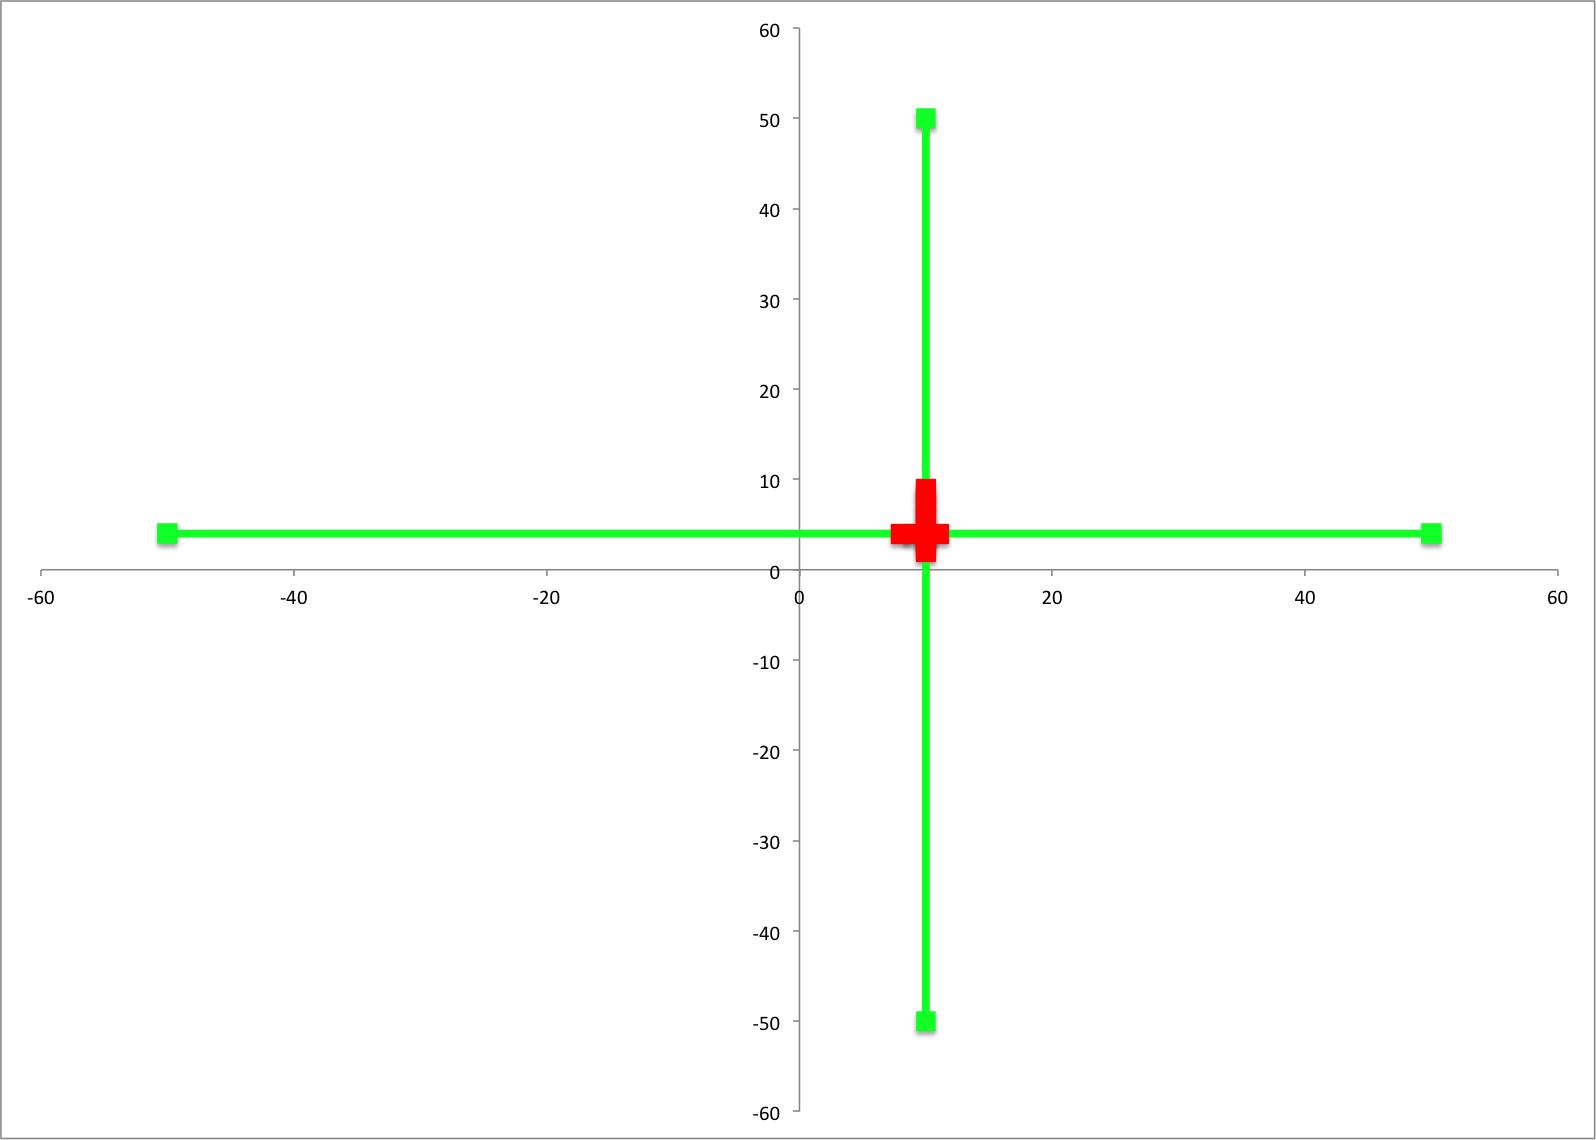
\includegraphics[width=0.49\linewidth]{excel_png/strip_pattern_A.png}}
%  end{center}
%\caption{Strip pattern failure domain}
%%  \label{fig:strip}
%\end{figure}

%Figure shows the example of strip pattern. Here we have two strip failure pattern for test 1 shown in \ref{fig1:a} and \ref{fig1:b} while 1 other for test 2 given in . The failure values are given in table .\\

\section{Implementation}
 The technique of automated discovery of failure domain is implemented in a tool called York Extensible Testing Infrastructure (YETI) \cite{Oriol2010a}. It is a testing tool developed in Java that test programs in an automated fashion using random strategies. YETI meta model is language-agnostic which enables it to test programs written in multiple languages that include Java, C\#, JML, .Net and Pharo. YETI consist of three main parts that include the core infrastructure responsible for extendibility through specialisation, the strategies to adjust multiple strategies and language-specific bindings to provide support for multiple languages \cite{Oriol2010}. The default test strategy for testing is simple random.

\begin{figure}[htp]
\centering
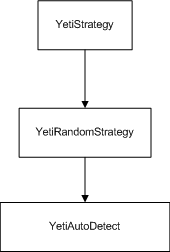
\includegraphics[width=3cm,height=4cm]{Hierarchy1.png}
\caption{Class Hierarchy of automated discovery of failure domains in YETI}
\label{fig:hierarchy}
\end{figure}

Strategies package contain all the strategies that can be selected for testing according to the specific needs. On top of the hierarchy is an abstract class YetiStrategy which is extended by YetiRandomStrategy and it is further extended to get YetiAutoDectect (ADFD) strategy as shown in figure \ref{fig:hierarchy}. 





\section{Conclusion}
One conclusion is that ARDT helps in exploring new faults or you can say new failure test cases because if you see figure 3 (a, b, c) it gives 3 range of values for which the program fails. \\

Doing this also saves time in debugging because in ordinary testing the testing stops as soon as the fault is discovered and once the fault is removed by the developers the testing starts again. But here the develop debug the program for all the range instead of single fault value thus saving multiple steps. \\


Debugging can also be made more efficient because the debugger will have the list of all the values for which the program fail therefore he will be in a more better position to rectify the faults and test them against those special values before doing any further testing.\\

We also found that the block and strip pattern are most common in arithmatic programs where as point pattern are more frequently found in general programs. \\

This study will also let us know the reality of failure patterns and its existence across the programs.


%ACKNOWLEDGMENTS are optional
\section{Acknowledgments}
This section is optional; it is a location for you
to acknowledge grants, funding, editing assistance and
what have you.  In the present case, for example, the
authors would like to thank Gerald Murray of ACM for
his help in codifying this \textit{Author's Guide}
and the \textbf{.cls} and \textbf{.tex} files that it describes.

%
% The following two commands are all you need in the
% initial runs of your .tex file to
% produce the bibliography for the citations in your paper.
\bibliographystyle{abbrv}
\bibliography{sigproc}  % sigproc.bib is the name of the Bibliography in this case
% You must have a proper ".bib" file
%  and remember to run:
% latex bibtex latex latex
% to resolve all references
%
% ACM needs 'a single self-contained file'!
%
%APPENDICES are optional
%\balancecolumns
\appendix
% That's all folks!
\end{document}
